\documentclass[12pt]{article}


\usepackage[hidelinks]{hyperref}

\usepackage[utf8]{inputenc}
\usepackage[T1]{fontenc}

\usepackage{graphicx}

% STIX for the text
\usepackage{stix}

% Inconsolata for the code
\usepackage{inconsolata}

\usepackage{amsmath}

% Helvetica for the titles
\usepackage[scaled]{helvet}

% Spacing
\usepackage{setspace}

% Track changes
\usepackage[inline]{trackchanges}
\usepackage{color}
\newcommand{\hilight}[1]{\colorbox{yellow}{#1}}


\addeditor{author.id}
\addeditor{author.id}


\usepackage[letterpaper]{geometry}
\geometry{margin=2.5cm}



\usepackage{lineno}
\linenumbers

%%% Syntax Highlighting for code  %%%
%%% Adapted from knitr book %%%
\usepackage{fancyvrb}
\DefineVerbatimEnvironment{Highlighting}{Verbatim}{commandchars=\\\{\}}
% Add ',fontsize=\small' for more characters per line
\newenvironment{Shaded}{}{}
\newcommand{\KeywordTok}[1]{\textcolor[rgb]{0.00,0.44,0.13}{\textbf{{#1}}}}
\newcommand{\DataTypeTok}[1]{\textcolor[rgb]{0.56,0.13,0.00}{{#1}}}
\newcommand{\DecValTok}[1]{\textcolor[rgb]{0.25,0.63,0.44}{{#1}}}
\newcommand{\BaseNTok}[1]{\textcolor[rgb]{0.25,0.63,0.44}{{#1}}}
\newcommand{\FloatTok}[1]{\textcolor[rgb]{0.25,0.63,0.44}{{#1}}}
\newcommand{\CharTok}[1]{\textcolor[rgb]{0.25,0.44,0.63}{{#1}}}
\newcommand{\StringTok}[1]{\textcolor[rgb]{0.25,0.44,0.63}{{#1}}}
\newcommand{\CommentTok}[1]{\textcolor[rgb]{0.38,0.63,0.69}{\textit{{#1}}}}
\newcommand{\OtherTok}[1]{\textcolor[rgb]{0.00,0.44,0.13}{{#1}}}
\newcommand{\AlertTok}[1]{\textcolor[rgb]{1.00,0.00,0.00}{\textbf{{#1}}}}
\newcommand{\FunctionTok}[1]{\textcolor[rgb]{0.02,0.16,0.49}{{#1}}}
\newcommand{\RegionMarkerTok}[1]{{#1}}
\newcommand{\ErrorTok}[1]{\textcolor[rgb]{1.00,0.00,0.00}{\textbf{{#1}}}}
\newcommand{\NormalTok}[1]{{#1}}
\usepackage{enumerate}
\usepackage{ctable}
\usepackage{float}


\providecommand{\tightlist}{%
	\setlength{\itemsep}{0pt}\setlength{\parskip}{0pt}}

\begin{document}

\setlength{\parskip}{1em}
\setlength{\parindent}{0pt}


{\Large\bfseries\sffamily Coevolution leaves a stronger imprint on interactions than on community
structure}
\vskip 2em


\href{http://orcid.org/0000-0002-0735-5184}{Timothée Poisot}
$^{1, 2, 3 ,\ast}$, %\\
Daniel B. Stouffer
$^{1 }$\bigskip

\small
(1) School of Biological Sciences, University of Canterbury, Christchurch,
New Zealand\\
(2) Département des Sciences Biologiques, Université de Montréal, Montréal,
Canada\\
(3) Québec Centre for Biodiversity Sciences, Montréal, Canada\\
\bigskip
\normalsize

 $\ast$ e-mail: \texttt{tim@poisotlab.io}

\bigskip

{\small
\textbf{Abstract: }Coevolutionary dynamics act on both species and their interactions in
ways that shape ecological communities. It remains unclear, however, how
the structure of communities at larger spatial scales either influences
or is influenced by local coevolutionary processes, and how mechanisms
acting at these different scales feedback onto one another. Here we show
that, although species interactions vary substantially over a
continental gradient, the coevolutionary significance of individual
interactions is maintained across different scales. Notably, this occurs
despite the fact that observed community variation at the local scale
frequently tends to weaken or remove community-wide coevolutionary
signal. When considered in terms of the interplay between community
ecology and coevolutionary theory, our results demonstrate that
individual interactions are capable and likely to show a consistent
signature of past coevolution even when woven into communities that do
not.
}\\
{\small
\textbf{Keywords:}
  markdown \,\,\,\,\,\,\,\,\,\,
  pandoc \,\,\,\,\,\,\,\,\,\,
  LaTeX \,\,\,\,\,\,\,\,\,\,
}

{\small
\textbf{Date: }
Work in progress.
}\vskip 1em

\clearpage
\doublespacing


Ecological interactions often exert important selective pressures on the
species involved. For example, the phenologies of lodgepole pines and
red crossbills respond spatially to the presence of squirrels (Benkman
et al. 2003) and palm species undergo changes in seed morphology in
response to the extinction of bird dispersing their seeds (Galetti et
al. 2013). Given that interactions are distributed in similar ways
across communities, at both the large or small scale (Jordano,
Bascompte, and Olesen 2003), it can be argued that much ecological
structure is the end result of evolutionary or coevolutionary dynamics
between species ({\textbf{???}}; Stouffer et al. 2012). Unfortunately,
while the coevolutionary dynamic of pairs of interacting species has
been well described at macro (Van Valen 1973) and micro (Gandon et al.
2008) evolutionary timescales, most attempts to understand how they
cascade up to the levels of diversity of both species and interactions
found within empirical communities have been inconclusive (Hembry,
Yoder, and Goodman 2014). Moreover, because coevolutionary dynamics are
often presented as a key driving force behind ecological structure
across both time and space (Thompson 2005), it is crucial to determine
the scale at which they are both relevant and quantifiable.

Historically, the evidence for coevolution in taxonomically diverse
communities is quantified as the degree of matching between the
phylogenies of two sets of interacting organisms (Legendre, Desdevises,
and Bazin 2002). This notion builds on the century-old idea that extant
species interact in a way similar to the way their ancestors did
(Fahrenholz 1913), but it is considerably more restrictive than just
phylogenetic conservation of species' interactions (Rezende et al. 2007;
{\textbf{???}}) because of additional higher-order constraints. More
explicitly, communities that have assembled by successive divergence
events due to coevolution should display phylogenetic congruence, that
is (i) have similar phylogenetic trees and (ii) have species at matching
positions in the trees that tend to interact (Page 2003). On the other
hand, many ecological and evolutionary processes that occur locally are
expected to blur community-wide coevolutionary signal (Poisot 2015). One
possible explanation is that interactions can display substantial
turnover at ecologically relevant temporal and spatial scales
({\textbf{???}}): the same two species can interact in different ways
under the effect of local environmental contingencies, spatial mismatch
in species phenologies, variations in population abundances, and chance
events ({\textbf{???}}). It is unclear, however, whether these
mechanisms influence how the coevolutionary signal within individual
interactions should vary across spatial scales.

\section{Methods}\label{methods}

\subsection{Data source and
pre-treatment}\label{data-source-and-pre-treatment}

We use data on observations of interactions between 121 species of
rodents and 205 species of parasitic fleas in 51 locations across Europe
({\textbf{???}}) to build 51 species-species interaction networks.
Interactions were measured by combing rodents for fleas, a method that
gives high quality data as it has a high power of detection. To account
for differential sampling effort and across site variations in
abundance, we only study the networks' incidence matrices (presence and
absence of interactions). Previous analyses revealed that this dataset
shows significant coevolutionary signal at the continental level {[}B.
R. Krasnov et al. (2012); \(p \leq 10^{-4}\), see Methods{]}.
Importantly, it also provides spatial replication and variability
({\textbf{???}}) at a scale large enough to capture macro-ecological
processes. This dataset is uniquely suited for our analysis, as it
represents a paradigmatic system in which species-species interactions
are thought to be driven by macro-evolution and co-speciation events
(Verneau, Du Preez, and Badets 2009).

The original dataset gives quantitative interaction strengths (expressed
as an averaged number of parasites per species per host). Quantitative
interactions strength, in this system, were shown to be affected to a
very high degree by local variations in abundance across sampling
locations ({\textbf{???}}), and it therefore seems unlikely that they
reflect macro-ecological processes. For this reason, we transform all
quantitative matrices into bipartite incidence matrices, in which 1
represents the presence of an interaction, and 0 its absence.

\subsection{Spatial scales and interaction spatial
consistency}\label{spatial-scales-and-interaction-spatial-consistency}

We define threes scales for the network data and their subsequent
analysis---continental, regional, and local. The continental scale is
the aggregated ``metanetwork'' which includes all documented
interactions between species from the regional species pool
({\textbf{???}}). Note that although they are reported as 0, we actually
have no information about species pairs that have never co-occured.

Within each site, the regional scale is given by the subset of
metanetwork formed by the locally present species. Hence the regional
networks are always a perfect subset of the continental network, and do
not reflect whether species were actually observed to interact locally
or not. By contrast, the local scale includes only the interactions that
were actually observed in the field at a given site. Therefore, the
local and regional networks always include the same species, but the
local network has only a subset (or, at most, an exact match) of the
interactions in the regional network.

We define the spatial consistency of every interaction as the number of
sites in which the two species involved co-occur. Note that, because of
the co-occurence issue mentioned above, this measure is only defined for
species that have been observed to \emph{interact} at least once.

\subsection{Measure of coevolutionary
signal}\label{measure-of-coevolutionary-signal}

We quantify the strength of coevolutionary signal in terms of the degree
of matching between host and parasite phylogenies, given knowledge of
species interactions. We do so using the \emph{PACo} method (Balbuena,
M{í}guez-Lozano, and Blasco-Costa 2013), which is robust to variations
in number of species and interactions. \emph{PACo} provides measures of
both the network-level congruence (\emph{i.e.}, is the network
coevolved?) and the interaction-level signal (\emph{i.e.}, what is the
contribution of each interaction to the overall coevolutionary signal?).
Importantly, and by contrast to previous methods such as \emph{ParaFit}
(Legendre, Desdevises, and Bazin 2002), \emph{PACo} allows measuring the
contribution of every interaction to the network-level signal even
though the network shows no significant coevolutionary signal. As
required by \emph{PACo}, the phylogenetic trees for hosts and parasites
were rendered ultrametric (\emph{i.e.}, all species are at the same
distance from the root).

\section{Results}\label{results}

\subsection{Local and regional scale networks show no coevolutionary
signal}\label{local-and-regional-scale-networks-show-no-coevolutionary-signal}

As host-macroparasite interactions are hypothesized to be both
ecologically constrained and evolutionary conserved (Combes 2001), the
congruence observed at the continental level sets the baseline for what
would be expected in local communities. Of course, if ecological
mechanisms reduce coevolutionary signal, we should detect coevolution at
the continental scale but not locally. Noting that variation of
interactions can decrease congruence, we analyse the data at two
different levels to test these hypotheses: first, we use \emph{regional}
interaction data---which accounts for different species composition
across sites--and second, we use the \emph{local} interaction
data---which also accounts for variation in the interactions between
observed these species (Methods Summary). Out of 51 sites, 35 show no
signal of coevolution, 11 show significant coevolutionary signal when
using the regional interactions, and 12 show significant coevolutionary
signal using the local interactions (see \emph{Supp. Mat. 1} for
network-level significance values; \autoref{maps}).

\subsection{Coevolutionary signal is predicted by the contribution of
interactions}\label{coevolutionary-signal-is-predicted-by-the-contribution-of-interactions}

These results would appear to support the idea that macro-evolutionary
processes such as co-diversification can have consequences at the
macro-ecological level but may not in fact be detectable at finer
spatial scales. On the other hand, system-level differences say little
about the behaviour of individual interactions, despite the fact most
coevolutionary mechanisms act at the interaction level (Thompson 1999).
As might be expected, we observe here that networks with interactions
that are important for coevolution at the continental scale indeed have
more coevolutionary signal at the local and regional scales alike (Fig.
2A). Intriguingly, we also find that the distribution of individual
interactions' contributions to coevolution is strongly conserved,
regardless of the scale at which the interactions are quantified (Fig.
2B). Because interactions differ in their total contribution to
coevolution, this implies that their distribution across networks is
what actually drives differences in overall coevolutionary signal.
Network-level coevolutionary signal emerges directly from the properties
of interactions and is not a property of the network itself.

\subsection{Interactions contributing to coevolution are not more
spatially
consistent}\label{interactions-contributing-to-coevolution-are-not-more-spatially-consistent}

Beyond their contribution to coevolution, interactions also ultimately
differ in how frequently they vary when the species involved co-occur
(Olito and Fox 2014). Once more, the literature on host-parasite
interactions usually assumes that the reason why some interactions are
more frequent is because they reflect a significant past history of
coevolution (Morand and Krasnov 2010). If this were true, we should
observe a significant, positive correlation between the probability of
observing an interaction and the importance of that interaction for
coevolution at the continental scale (Methods Summary). Surprisingly, we
find that neither is true here since interactions that are important for
coevolution are not more conserved (Fig. 3).

\subsection{The contribution of interactions to coevolution is
consistent across
scales}\label{the-contribution-of-interactions-to-coevolution-is-consistent-across-scales}

Ultimately, coevolutionary signal varies across scale because of the
simultaneous variation of species' interactions \emph{and} communities'
phylogenetic tree structure. In a system characterised by substantial
turnover, we would expect the contribution of each separate interaction
to differ across scales as well. Instead, we observe here that
interactions that contribute strongly to coevolutionary signal at the
continental scale \emph{also} show a significant tendency to contribute
strongly at the local (\(p<0.05\) for positive correlations in 48 out of
51 networks) and regional (in 47 out of 51 networks), and this
observation is independent of network-wide coevolutionary signal (Fig.
4). Remarkably, this result implies that the remnants of coevolution are
still locally detectable in \emph{individual interactions} even though
coevolution regularly fails to leave its imprint on most local networks.

\section{Discussion}\label{discussion}

Overall, the results of our analyses demonstrate that there is a
sizeable gap between our current understanding of coevolution as the
basis of multi-species interactions and its applicability to ecological
questions. Local networks show little to no signal of coevolution and
the strength of coevolution between two species is a surprisingly poor
predictor of how frequently they interact. In contrast to the frequent
assumption that phylogenetic structure is a key driver of community
structure (Cavender-Bares et al. 2009), these data reveal that this
impact is actually minimal at ecologically relevant spatial scales.
Despite all the above, individual interactions are able to maintain
their coevolutionary signal even when the community they are woven into
does not. Thinking more broadly, these discrepancies provide a clear
roadmap for bridging the aforementioned gap between our appreciation of
the role of coevolution and its empirically measurable outcomes. Network
structure is the most parsimonious \emph{mechanism} by which coevolution
proceeds, not the imprint coevolution leaves on ecological communities.

\textbf{Acknowledgements.} We thank Juan Antonio Balbuena for
discussions about the \emph{PACo} method, and members of the Stouffer
and Tylianakis groups for comments on an early draft of this manuscript.
We are indebted to Matt Hutchinson and Fernando Cagua for contributions
to the code of the \texttt{paco} R package. Funding to TP and DBS was
provided by a Marsden Fund Fast-Start grant (UOC-1101) and to DBS by a
Rutherford Discovery Fellowship, both administered by the Royal Society
of New Zealand.

\section*{References}\label{references}
\addcontentsline{toc}{section}{References}

Balbuena, Juan Antonio, Ra{ú}l M{í}guez-Lozano, and Isabel Blasco-Costa.
2013. ``PACo: A Novel Procrustes Application to Cophylogenetic
Analysis.'' \emph{PLoS ONE} 8 (4): e61048.

Benkman, Craig W., Thomas L. Parchman, Amanda Favis, and Adam M.
Siepielski. 2003. ``Reciprocal Selection Causes a Coevolutionary Arms
Race Between Crossbills and Lodgepole Pine.'' \emph{Am. Nat.} 162 (2):
182--94.

Cavender-Bares, Jeannine, Kenneth H. Kozak, Paul V. A. Fine, and Steven
W. Kembel. 2009. ``The Merging of Community Ecology and Phylogenetic
Biology.'' \emph{Ecol. Lett.} 12 (7): 693--715.

Combes, Claude. 2001. \emph{Parasitism - The Ecology and Evolution of
Intimate Interactions}. University Of Chicago Press.

Fahrenholz, H. 1913. ``Ectoparasiten Und Abstammungslehre.'' \emph{Zool.
Anz.} 41: 371--74.

Galetti, Mauro, Roger Guevara, Marina C. C{ô}rtes, Rodrigo Fadini,
Sandro Von Matter, Abra{ã}o B. Leite, F{á}bio Labecca, et al. 2013.
``Functional Extinction of Birds Drives Rapid Evolutionary Changes in
Seed Size.'' \emph{Science} 340 (6136): 1086--90.

Gandon, Sylvain, Angus Buckling, Ellen Decaestecker, and Troy Day. 2008.
``Host-Parasite Coevolution and Patterns of Adaptation Across Time and
Space.'' \emph{J. Evol. Biol.} 21 (6): 1861--66.

Hembry, David H., Jeremy B. Yoder, and Kari Roesch Goodman. 2014.
``Coevolution and the Diversification of Life.'' \emph{The American
Naturalist} 184 (4): 425--38.

Jordano, Pedro, Jordi Bascompte, and Jens M Olesen. 2003. ``Invariant
Properties in Coevolutionary Networks of Plant-Animal Interactions.''
\emph{Ecol. Lett.} 6 (1): 69--81.

Krasnov, Boris R., Miguel A. Fortuna, David Mouillot, Irina S.
Khokhlova, Georgy I. Shenbrot, and Robert Poulin. 2012. ``Phylogenetic
Signal in Module Composition and Species Connectivity in
Compartmentalized Host-Parasite Networks.'' \emph{The American
Naturalist} 179 (4): 501--11.

Legendre, Pierre, Yves Desdevises, and Eric Bazin. 2002. ``A Statistical
Test for Host-Parasite Coevolution.'' \emph{Syst. Biol.} 51 (2):
217--34.

Morand, Serge, and Boris Krasnov, eds. 2010. \emph{Biogreography of
Host-Parasite Interactions}. Oxford: Oxford University Press.

Olito, Colin, and Jeremy W. Fox. 2014. ``Species Traits and Abundances
Predict Metrics of Plantpollinator Network Structure, but Not Pairwise
Interactions.'' \emph{Oikos}, n/a--/a.

Page, Roderick D M. 2003. \emph{Tangled Trees: Phylogeny, Cospeciation,
and Coevolution}. University of Chicago Press.

Poisot, Timoth{é}e. 2015. ``When Is Cophylogeny Evidence of
Coevolution?'' In \emph{Evolutionary Ecology of Host-Parasite Systems},
edited by Serge Morand, D T Littlewood, and Robert Poulin. Cambridge
University Press.

Rezende, Enrico L, Jessica E Lavabre, Paulo R Guimar{ã}es, Pedro
Jordano, and Jordi Bascompte. 2007. ``Non-Random Coextinctions in
Phylogenetically Structured Mutualistic Networks.'' \emph{Nature} 448
(7156): 925--8.

Stouffer, Daniel B., Marta Sales-Pardo, M. Irmak Sirer, and Jordi
Bascompte. 2012. ``Evolutionary Conservation of Species' Roles in Food
Webs.'' \emph{Science} 335 (6075): 1489--92.

Thompson, John N. 1999. ``The Raw Material for Coevolution.''
\emph{Oikos} 84 (1): 5--16.

---------. 2005. \emph{The Geographic Mosaic of Coevolution}. University
Of Chicago Press.

Van Valen, Leigh. 1973. ``A New Evolutionary Law.'' \emph{Evol. Theory}
1 (1): 1--30.

Verneau, Olivier, Louis Du Preez, and Mathieu Badets. 2009. ``Lessons
from Parasitic Flatworms About Evolution and Historical Biogeography of
Their Vertebrate Hosts.'' \emph{C. R. Biol.} 332 (2): 149--58.

\singlespacing

\clearpage
\listoffigures
\clearpage
\begin{figure}[p!]
  \centering
  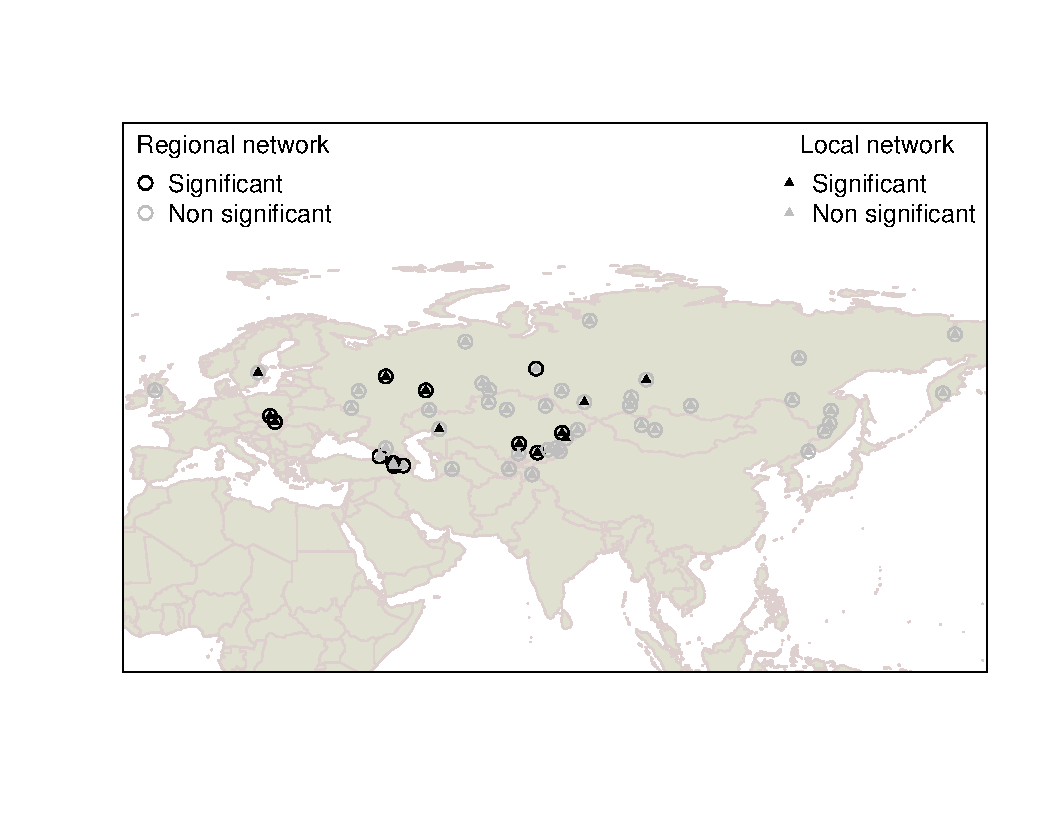
\includegraphics[width=\textwidth]{../figures/figure1.pdf}
	\caption[Spatial distribution.]{Spatial distribution of coevolutionary signal across the 51 sites. For
each location, we indicate whether or not the structure of regional and
local interaction networks is consistent with phylogenetic congruence.
The colour of the circle corresponds to regionally significant or
non-significant (black and grey, respectively) while the colour of the
symbol within corresponds to locally significant or non-significant
(black and grey, respectively).}
	\label{maps}
\end{figure}
\cleardoublepage
\begin{figure}[p!]
  \centering
  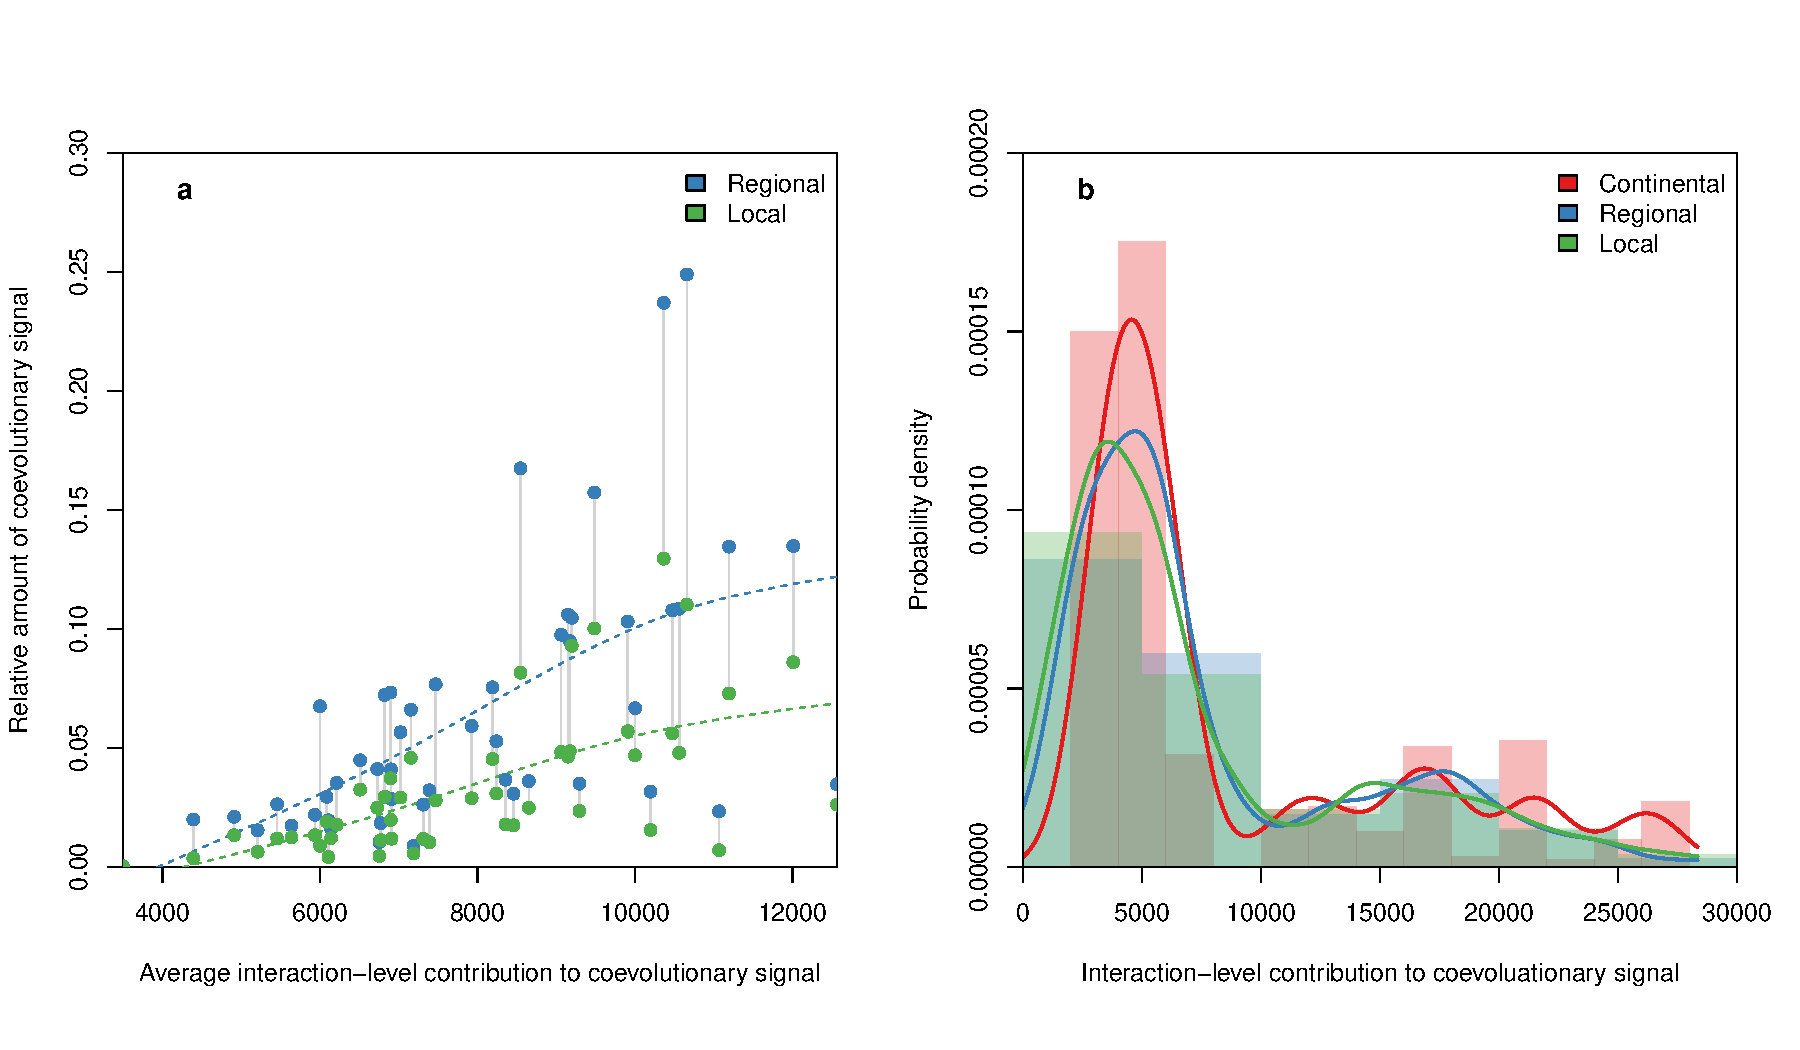
\includegraphics[width=\textwidth]{../figures/figure4.pdf}
	\caption[Example figure.]{Distribution of coevolutionary signal at the network and interaction
levels. \textbf{a}, Networks that have lower coevolutionary signal at
the local or regional level are composed of interactions that on average
contribute little to coevolution at the continental scale. Dashed lines
are the cubic smoothing spline; the two levels of the same networks are
linked by solid grey lines. \textbf{b}, Overall, interactions observed
at the local, regional, and continental scale have equal contributions
to coevolutionary signal. Probability density was smoothed using a
Gaussian kernel density estimator. Raw probability densities are shown
as semi-transparent bars.}
	\label{contributions}
\end{figure}
\cleardoublepage
\begin{figure}[p!]
  \centering
  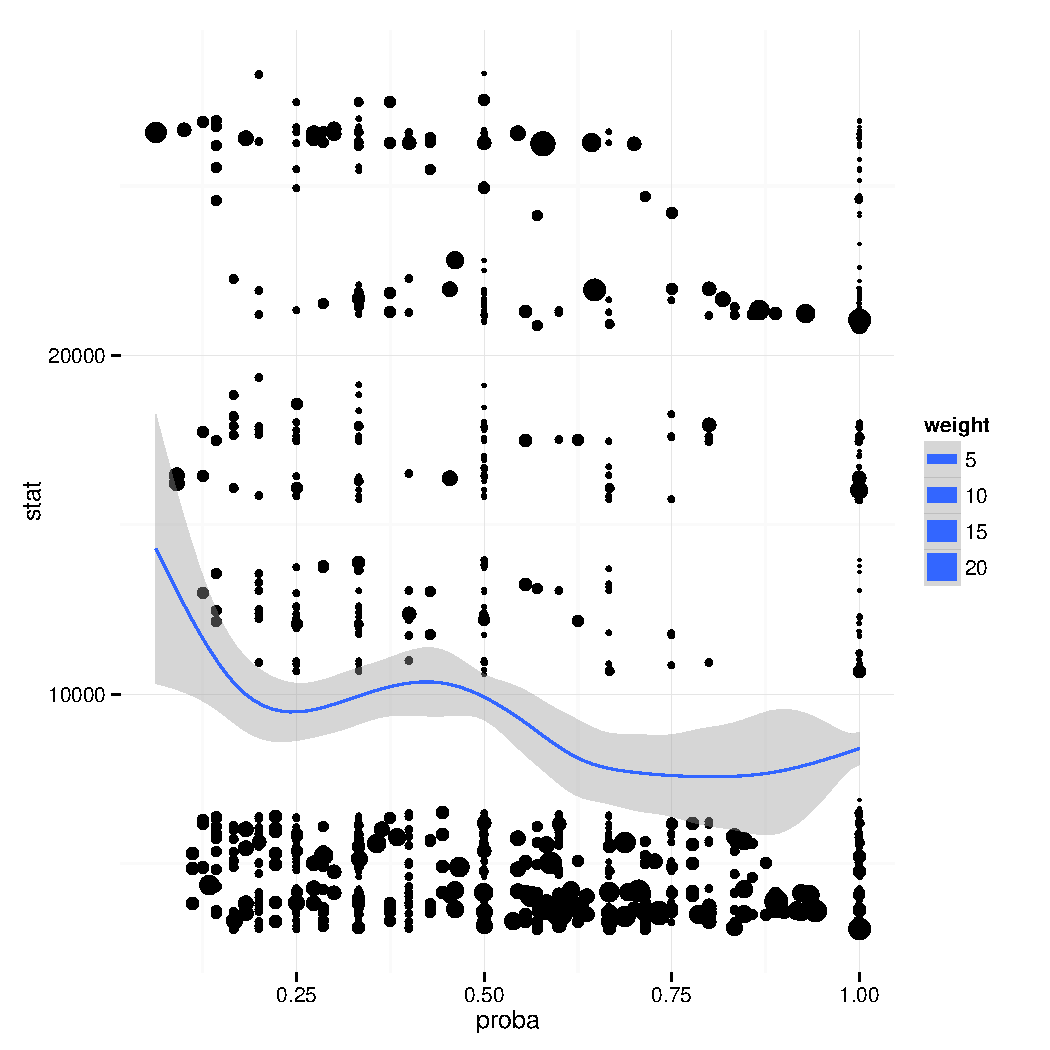
\includegraphics[width=\textwidth]{../figures/figure3.pdf}
	\caption{Spatial consistency of an interaction and its contribution to
coevolutionary signal. Spatial consistency is defined as the probability
of observing an interaction between two species given that they were
observed to co-occur. Although statistically significant, there was no
biologically meaningful relationship between spatial consistency and an
interaction's importance for coevolution in the continental network
(\(R^2 \approx 0.01\), \(\rho = -0.1\), \(p \leq 10^{-5}\)).}
	\label{consistency}
\end{figure}
\cleardoublepage
\begin{figure}[p!]
  \centering
  \includegraphics[width=\textwidth]{../figures/figure2.pdf}
	\caption{The contribution to coevolutionary signal of the interaction between two
species is maintained across scales. For every site, we show the
Pearson's correlation between interaction-level coevolutionary signal in
the continental network and the same in the local network. The size of
each point is proportional to the size of the network, and all
correlations are significant at \(\alpha = 0.05\) except in the grey
shaded area.}
	\label{scales}
\end{figure}
\cleardoublepage


\end{document}
